\chapter*{Serie 1}
First lets do a sketch as seen in figure \ref{fig:sp} to omit any misunderstanding of the problem.
\begin{figure}[]
	\begin{center}
		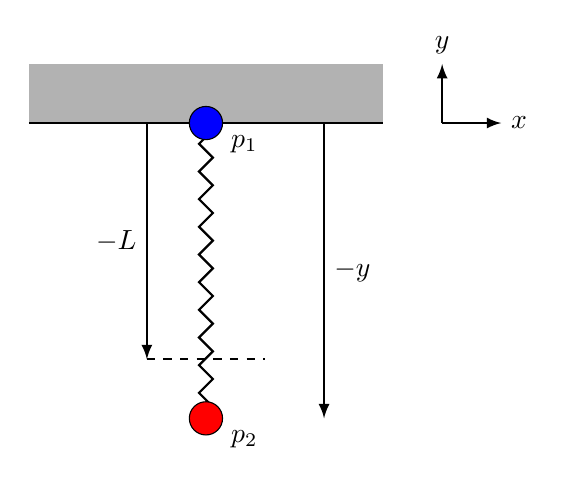
\begin{tikzpicture}[decoration=zigzag, mass/.style={label distance=2mm},scale=1.5]
			\fill[black!30] (-1.5,0) rectangle (1.5,0.5);
			\draw[thick] (-1.5,0) -- (1.5,0);
			\begin{scope}[shift={(2,0)}]
				\coordinate[label=above:$y$,thick] (y) at (0,0.5);
				\coordinate[label=right:$x$,thick] (x) at (0.5,0);
				\draw[-latex,thick] (0,0) -- (y);
				\draw[-latex,thick] (0,0) -- (x);
			\end{scope}
			\coordinate[label={[mass]350:$p_1$}] (m1) at (0,0);
			\coordinate[label={[mass]350:$p_2$}] (m2) at (0,-2.5);
			\draw[decorate,thick] (m1) -- (m2);
			\fill[blue,draw=black] (m1) circle (4pt);
			\fill[red,draw=black] (m2) circle (4pt);
			\path[-latex,draw,thick] (-0.5,0) to[left] node{$-L$} (-0.5,-2);
			\path[-latex,draw,thick] (1,0) to[right] node{$-y$} (1,-2.5);
			\draw[dashed,thick] (-0.5,-2) -- (0.5,-2);
		\end{tikzpicture}
	\end{center}
	\caption{Sketch of the spring problem, $p_2$ being not in rest state.}
	\label{fig:sp}
\end{figure}
We would like to find the constants $c_1, c_2$ of the equation
\begin{align}
	y(t)&=c_1 e^{\alpha t}\cos (\beta t)+c_2 e^{\alpha t}\sin(\beta t) - L -\frac{mg}{k},
	\label{eq:gf}
	\intertext{where the constraints are the rest state initial conditions, which means there is no energy in the system except gravitational energy at $t=0$. This has the same physical meaning as the spring having its rest length $L$ \footnote{if there would be no other force than the one of the feather} and no kinetic energy at $t=0$. This can be expressed as}
	 y(t=0) &= -L,
	\label{eq:c1a}
	\shortintertext{and}
		\dot{y}(t=0)&=0.
	\label{eq:c2a}
	 \intertext{The position of $p_2$ computed with the given solution Eq. \ref{eq:gf} is}
	 y(t=0) &= c_1-L-\frac{mg}{k}.
	\label{eq:c1b}
	\intertext{Comparing Eq. \ref{eq:c1a} and Eq. \ref{eq:c1b} gives us}
	c_1&=\frac{mg}{k}.
	\intertext{To get $c_2$ we need to compute $\dot{y}(t=0)$ from  Eq. \ref{eq:gf}}
	\dot{y}(t=0)&=\!\left( c_1\alpha +c_2 \beta -L -\frac{mg}{k} \right),
	\shortintertext{where $c_1=mg/k$ leads to}
	\dot{y}(t=0)&= \frac{mg}{k}\alpha +c_2\beta -L-\frac{mg}{k}.
	\intertext{Using the constraint in Eq. \ref{eq:c2a} finally gives us}
	c_2&=\frac{mg}{\beta k}(1-\alpha)+\frac{L}{\beta}.
\end{align}
